\documentclass[11pt]{article}
\usepackage[margin=1in]{geometry}
\usepackage[T1]{fontenc}
\usepackage[utf8]{inputenc}
\usepackage{lmodern,booktabs,graphicx,longtable,amsmath,hyperref,parskip}
\hypersetup{colorlinks=true,urlcolor=blue}
\title{Years From Posed To Resolved: The Solvability Atlas\\\large MAT 124 Statistics Project}
\author{Gianangelo Dichio}
\date{2026-10-13}
\begin{document}
\maketitle


\section*{Abstract}
\noindent\fbox{\parbox{0.97\linewidth}{\textbf{DRAFT for Gianangelo to rewrite in his own words. Target 100 to 150 words.}}}

\medskip
Objective: estimate the mean number of years a research problem stays open, from the year it was posed to the year it was resolved, for the solved problems in the Solvability Atlas. The data are 294 cleaned rows from the atlas problem table built on 2026-10-13, one row per solved problem with both years recorded. Descriptive work used all 294 rows; inference used a sample of 50 rows drawn with replacement from the cleaned records under seed 124. The full-data mean is 31.71 years and the median is 20.00 years. Year posed and years to resolve have $r = -0.67$ and $R^2 = 0.45$. The 95\% t interval from the sample is 15.72 to 28.92 years. The two-sided test of $\mu = 50$ gives $t = -8.43$ and $p < 0.0001$, so the sample provides evidence against the benchmark at $\alpha = 0.05$.


\section{Data Form}

\textbf{Approval.} The assignment lists approved public sources. This dataset is the author's own and sits outside that list, so the instructor's approval of the source is pending. Assignment 1 asks for three dataset choices; this form covers the first choice, and the second and third choices are still to be added.

\textbf{Source line.} Solvability Atlas problem table, Bucket Foundation; code MIT, each row under the licence in its \texttt{licence} column (CC BY-SA 4.0 for Wikipedia rows, Apache-2.0 for formal-conjectures rows, MIT for atlas rows, and four rows that cite an AAAS headline); download: \url{https://github.com/bucket-foundation/bucket-foundation/blob/dev/tools/solvability-atlas/surface/table.csv}.

\textbf{Source.} Title: Solvability Atlas problem table. Creator: Bucket Foundation, Gianangelo Dichio. Accessed 2026-10-13. Data period: problems posed from 1506 to 2023 and resolved from 1676 to 2026. Files attached: \texttt{data/original.csv} and \texttt{data/cleaned.csv}.

\textbf{Population.} Solved research problems recorded in the atlas with a posed year and a resolved year. One row is one problem. The file holds 5209 problems, open and solved, compiled from public problem lists.

\textbf{Collection.} Observational. The rows were compiled from public lists: Wikipedia problem lists, science timelines and prize competition pages, the formal-conjectures repository and the atlas's own 71 curated problems. The sampling method of those lists is not reported. Limits on representation: a list favours well-known problems, and a problem enters this study only when both of its years were recorded, which leaves out most rows.

\textbf{Variables.} X: year posed, calendar year, quantitative, interval level. Y: years from posed to resolved, in years, quantitative, ratio level. Category 1: branch, with labels applied, biophysics, chemistry, cosmology, information, mathematics, mind, physics; categorical, nominal. Category 2: formal status, the state of a machine-checked proof, with labels none, partial, proved, statement; categorical, ordinal.

\textbf{Feasibility.} Total rows: 5209. Rows complete on the four variables after the filters: 294. Filters and missing-value rules are the seven cleaning rules in the Data Check. No category is derived.

\textbf{Question.} For solved research problems in the cleaned atlas table, is the mean time from posed to resolved equal to 50 years? Expected relationship: problems posed later have fewer years to resolve, because a recently posed problem that is already solved cannot have been open for long.

\textbf{Hypotheses.} $H_0: \mu = 50$ years. $H_1: \mu \ne 50$ years. The benchmark of 50 years is hypothetical. It was fixed in the code before the sample was drawn, and it stands for two research generations of 25 years each.

\section{Descriptive Statistics}

\subsection{Data Check}

Original rows: 5209. Removed: 4915. Retained: 294. Row IDs are the atlas \texttt{id} values and are kept in every file. Rules apply in order, and a row is counted under the first rule it meets. The excluded row IDs, one per line with the rule, are in \texttt{data/excluded\_rows.csv}.

\begin{center}\begin{tabular}{lr}
\toprule
Cleaning rule & Rows removed \\
\midrule
R1 posed year missing & 4201 \\
R2 resolved year missing & 710 \\
R3 status other than solved & 2 \\
R4 variant of another row & 2 \\
R5 resolved year before posed year & 0 \\
R6 branch or formal status missing & 0 \\
R7 duplicate id & 0 \\
\bottomrule
\end{tabular}\end{center}

Missing values: a row missing either year is removed under R1 or R2, and no value is imputed. Duplicate records: no ID repeats, and a variant row that restates part of another problem is removed under R4. Implausible values: a resolved year earlier than the posed year would be removed under R5, and no row met that rule.

\subsection{Tables}

Counts and relative frequencies of branch, denominator 294 problems.

\begin{center}\begin{tabular}{lrr}
\toprule
Branch & Count & Relative frequency \\
\midrule
mathematics & 117 & 0.3980 \\
physics & 46 & 0.1565 \\
information & 36 & 0.1224 \\
cosmology & 28 & 0.0952 \\
applied & 26 & 0.0884 \\
biophysics & 20 & 0.0680 \\
chemistry & 14 & 0.0476 \\
mind & 7 & 0.0238 \\
Total & 294 & 1.0000 \\
\bottomrule
\end{tabular}\end{center}

Counts and relative frequencies of formal status, denominator 294 problems.

\begin{center}\begin{tabular}{lrr}
\toprule
Formal status & Count & Relative frequency \\
\midrule
none & 197 & 0.6701 \\
proved & 87 & 0.2959 \\
statement & 7 & 0.0238 \\
partial & 3 & 0.0102 \\
Total & 294 & 1.0000 \\
\bottomrule
\end{tabular}\end{center}

Branch by formal status. Each cell holds the count and, in parentheses, the conditional row proportion; the denominator is the row total for that branch.

\begin{center}\begin{tabular}{lrrrrr}
\toprule
Branch & none & partial & proved & statement & Row total \\
\midrule
applied & 26 (1.0000) & 0 (0.0000) & 0 (0.0000) & 0 (0.0000) & 26 \\
biophysics & 20 (1.0000) & 0 (0.0000) & 0 (0.0000) & 0 (0.0000) & 20 \\
chemistry & 14 (1.0000) & 0 (0.0000) & 0 (0.0000) & 0 (0.0000) & 14 \\
cosmology & 28 (1.0000) & 0 (0.0000) & 0 (0.0000) & 0 (0.0000) & 28 \\
information & 32 (0.8889) & 0 (0.0000) & 4 (0.1111) & 0 (0.0000) & 36 \\
mathematics & 24 (0.2051) & 3 (0.0256) & 83 (0.7094) & 7 (0.0598) & 117 \\
mind & 7 (1.0000) & 0 (0.0000) & 0 (0.0000) & 0 (0.0000) & 7 \\
physics & 46 (1.0000) & 0 (0.0000) & 0 (0.0000) & 0 (0.0000) & 46 \\
Column total & 197 & 3 & 87 & 7 & 294 \\
\bottomrule
\end{tabular}\end{center}

Grouped Y. Classes are $[\text{lower}, \text{upper})$ in years. Sturges' rule gives $1 + \log_2 294 = 9.20$, about nine classes; the range of 387 years over nine classes is 43.00 years, rounded to a width of 40 years so that boundaries fall on multiples of 40.

\begin{center}\begin{tabular}{lrrrrr}
\toprule
Class, years & Midpoint & Count & Rel. freq. & Cum. count & Cum. rel. freq. \\
\midrule
0 to under 40 & 20 & 209 & 0.7109 & 209 & 0.7109 \\
40 to under 80 & 60 & 66 & 0.2245 & 275 & 0.9354 \\
80 to under 120 & 100 & 12 & 0.0408 & 287 & 0.9762 \\
120 to under 160 & 140 & 2 & 0.0068 & 289 & 0.9830 \\
160 to under 200 & 180 & 1 & 0.0034 & 290 & 0.9864 \\
200 to under 240 & 220 & 0 & 0.0000 & 290 & 0.9864 \\
240 to under 280 & 260 & 0 & 0.0000 & 290 & 0.9864 \\
280 to under 320 & 300 & 0 & 0.0000 & 290 & 0.9864 \\
320 to under 360 & 340 & 2 & 0.0068 & 292 & 0.9932 \\
360 to under 400 & 380 & 2 & 0.0068 & 294 & 1.0000 \\
\bottomrule
\end{tabular}\end{center}

\subsection{Summaries}

Y is years from posed to resolved. Variance uses the $n - 1$ denominator. Quartiles and the percentile follow QUARTILE.INC and PERCENTILE.INC, which is linear interpolation in \texttt{numpy.percentile}.

\begin{center}\begin{tabular}{lr}
\toprule
Statistic & Value, years \\
\midrule
n & 294 \\
Mean & 31.71 \\
Median & 20.00 \\
Mode & 0 (16 rows each) \\
Sample variance & 2223.61 \\
Sample standard deviation & 47.16 \\
Minimum & 0.00 \\
Q1 & 6.00 \\
Median & 20.00 \\
Q3 & 43.75 \\
Maximum & 387.00 \\
Range & 387.00 \\
IQR & 37.75 \\
90th percentile & 63.00 \\
\bottomrule
\end{tabular}\end{center}

Fences: lower $= Q1 - 1.5 \times IQR = 6.00 - 1.5(37.75) = -50.62$; upper $= Q3 + 1.5 \times IQR = 43.75 + 1.5(37.75) = 100.38$. Flagged outliers: 9. Row IDs with their values: \texttt{fermat} (357), \texttt{fourcolor} (124), \texttt{kepler} (387), \texttt{wp-caratheodory-conjecture-for-surfaces-of-smoothness-c-4-brend} (101), \texttt{sd-anthrax-as-a-microbial-disease} (330), \texttt{sd-collapse-of-a-massive-star-into-a-black-hole} (143), \texttt{sd-rings-of-uranus} (188), \texttt{sd-proton-as-a-nuclear-constituent} (104), \texttt{sd-colour-of-the-sky} (365).

With the flagged rows: mean 31.71, sample SD 47.16, n = 294. Without them: mean 25.35, sample SD 23.18, n = 285. Both results are kept, and every later calculation uses all 294 rows.

z-score for \texttt{fermat} (Fermat's Last Theorem): $z = (357 - 31.71) / 47.16 = 6.90$. This problem stayed open 6.90 sample standard deviations above the mean.

Within 1, 2 and 3 sample SDs of the mean: 0.9252, 0.9796 and 0.9830 of rows as proportions. The histogram is right-skewed with skewness 4.89, and the mean minus one SD is negative while Y has a floor of zero, so a bell-shaped model fits poorly; the proportions sit well above 0.68 at 1 SD and below 0.997 at 3 SDs. Chebyshev's theorem guarantees at least 75\% within 2 SDs for any distribution, and the data show 0.9796.

From class midpoints: mean 38.23 and sample SD 45.37, against 31.71 and 47.16 from the raw data. The differences are $6.52$ and $-1.79$ years.

\begin{center}\begin{tabular}{lrr}
\toprule
Branch & Count & Mean Y, years \\
\midrule
applied & 26 & 20.69 \\
biophysics & 20 & 33.20 \\
chemistry & 14 & 25.93 \\
cosmology & 28 & 32.39 \\
information & 36 & 18.64 \\
mathematics & 117 & 37.85 \\
mind & 7 & 44.29 \\
physics & 46 & 31.35 \\
\bottomrule
\end{tabular}\end{center}

Weighted mean of the branch means: $26(20.69) + 20(33.20) + 14(25.93) + 28(32.39) + 36(18.64) + 117(37.85) + 7(44.29) + 46(31.35)$, divided by 294, equals 31.71. The overall mean is 31.71, so the two agree.

\subsection{Relationships}

Paired count: 294. $r = -0.67$. Regression equation: $\hat y = 834.38 + (-0.41)x$, with x the year posed and $\hat y$ the years to resolve. $R^2 = 0.45$. Sum of squared residuals: 360782.10.

Slope: each later posed year goes with 0.41 fewer years to resolve on average. Intercept: 834.38 years is the fitted value at year 0, far outside the observed years 1506 to 2023, so it has no practical reading. $R^2$: year posed accounts for 44.62\% of the variation in years to resolve. The relationship is negative, roughly linear at the old end and weak to moderate in strength. The residuals fan out: they are wide for problems posed before 1900 and narrow for recent ones, and they are bounded below because Y cannot be negative.

Prediction at x = 1950, inside the observed range: $\hat y = 834.38 + (-0.41)(1950) = 29.85$ years. For \texttt{fermat} (Fermat's Last Theorem): x = 1637, observed y = 357, fitted 158.99, residual 198.01 years.

Extrapolation: the line gives negative years for posed years after 2022, so it cannot be used beyond the data. Possible confounder: branch, since older rows come from mathematics and physics. Causal limit: the data are observational and hold solved problems only. A problem posed in 2010 can appear here with at most 16 years, so part of the negative slope comes from which rows can be in the table, and no causal claim follows.

\subsection{Graphs And Interpretation}

\begin{center}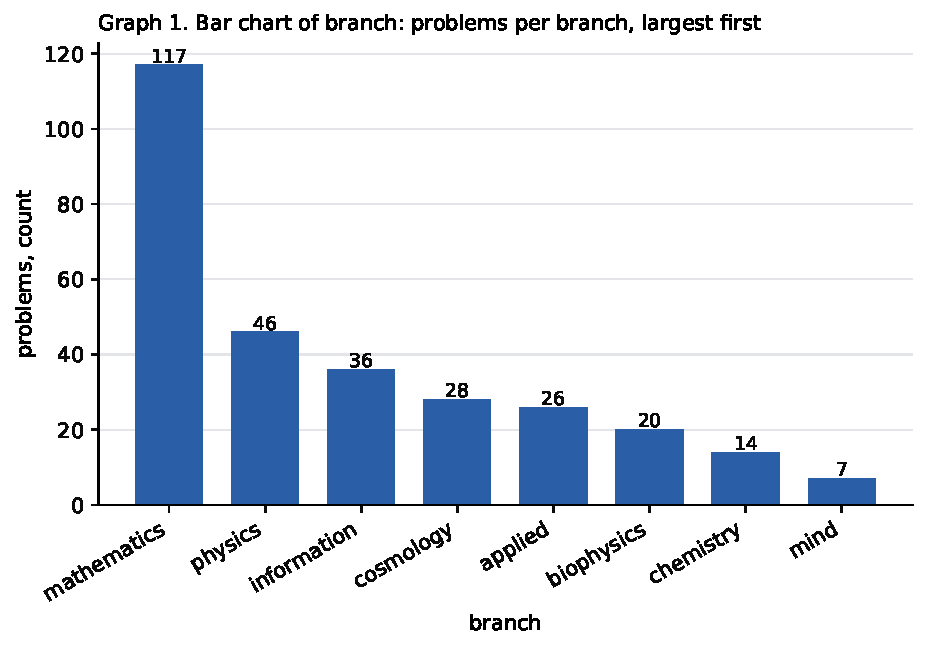
\includegraphics[width=0.82\linewidth]{figures/01-bar.pdf}\end{center}
\noindent Graph 1: mathematics has the most problems, 117, and mind the fewest, 7.


\begin{center}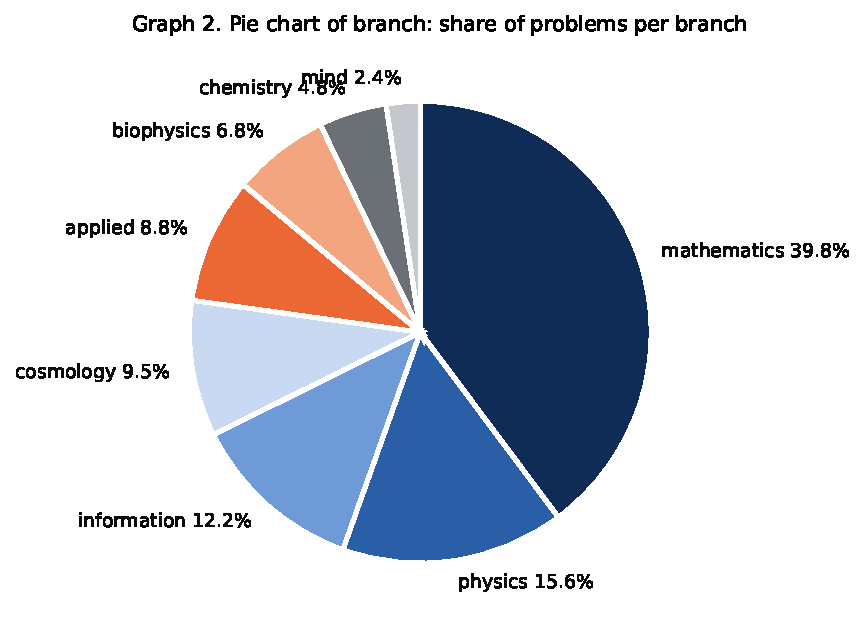
\includegraphics[width=0.82\linewidth]{figures/02-pie.pdf}\end{center}
\noindent Graph 2: the two largest branches, mathematics and physics, hold 55.44\% of the problems.


\begin{center}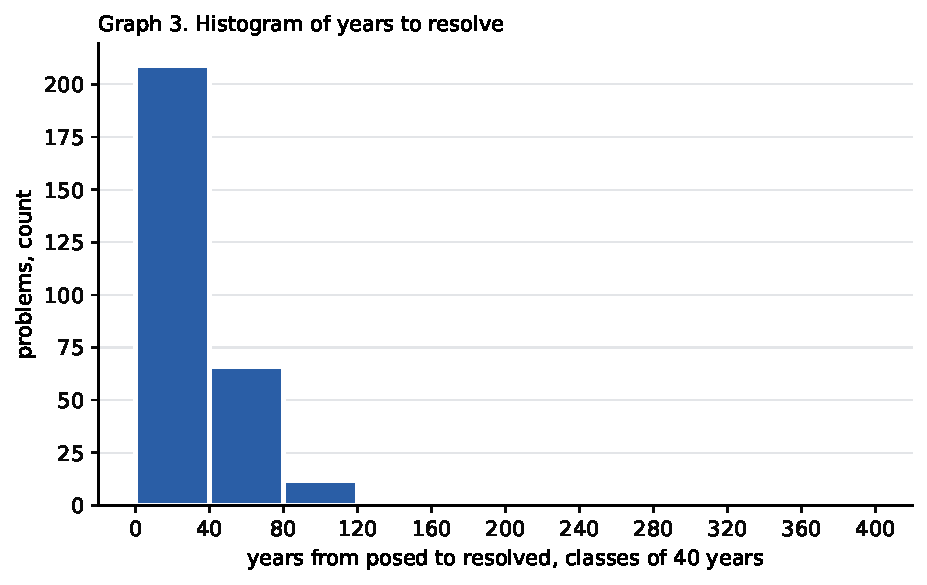
\includegraphics[width=0.82\linewidth]{figures/03-histogram.pdf}\end{center}
\noindent Graph 3: 209 of 294 problems fall in the first class, and counts drop off to a long right tail.


\begin{center}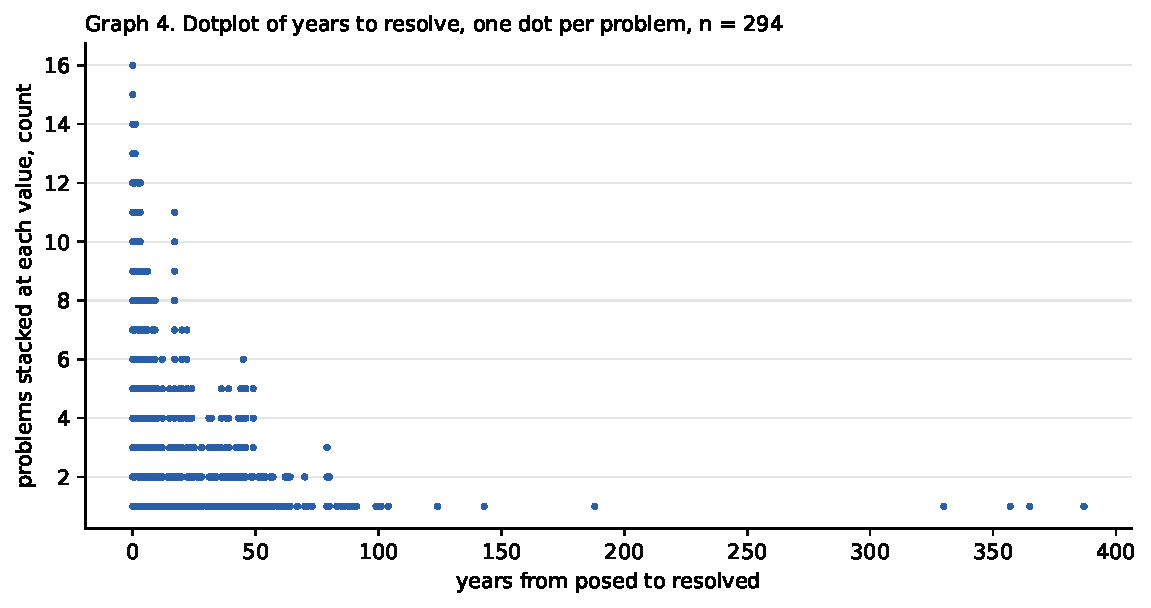
\includegraphics[width=0.82\linewidth]{figures/04-dotplot.pdf}\end{center}
\noindent Graph 4: the dots pile up from 0 to about 44 years, thin out by 100, and leave gaps before the largest values.


\noindent Graph 5. Stem plot of years to resolve. Key: \texttt{12 | 3} means 123 years; the stem is tens of years and each leaf is one problem.
\begin{footnotesize}\begin{verbatim}
  0 | 000000000000000011111111111111222222222222333333333333444444444555555555666666666777778888888899999999
  1 | 000001112222223445555566777777777778899999
  2 | 0000000122222223333444445556677888
  3 | 0111122223344456666677888899999
  4 | 00112223333444445555556666678899999
  5 | 011223344566779
  6 | 012233447
  7 | 0013999
  8 | 0035689
  9 | 19
 10 | 014
 11 | 
 12 | 4
 13 | 
 14 | 3
 15 | 
 16 | 
 17 | 
 18 | 8
 19 | 
 20 | 
 21 | 
 22 | 
 23 | 
 24 | 
 25 | 
 26 | 
 27 | 
 28 | 
 29 | 
 30 | 
 31 | 
 32 | 
 33 | 0
 34 | 
 35 | 7
 36 | 5
 37 | 
 38 | 7
\end{verbatim}\end{footnotesize}
\noindent Graph 5: 284 of 294 leaves sit on stems 0 to 9, and stems 20 to 32 are empty.

\begin{center}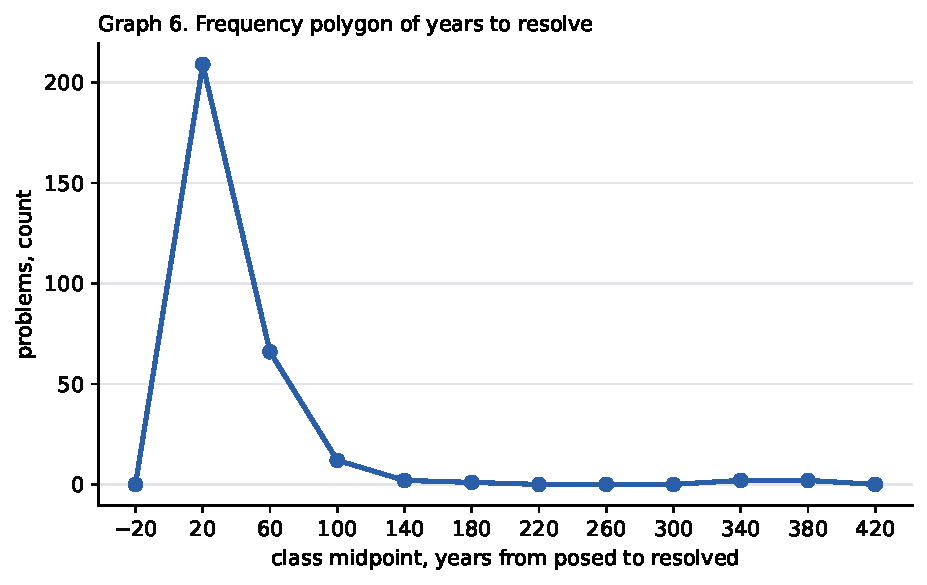
\includegraphics[width=0.82\linewidth]{figures/06-polygon.pdf}\end{center}
\noindent Graph 6: the polygon peaks at the first midpoint, 20 years, and falls steeply.


\begin{center}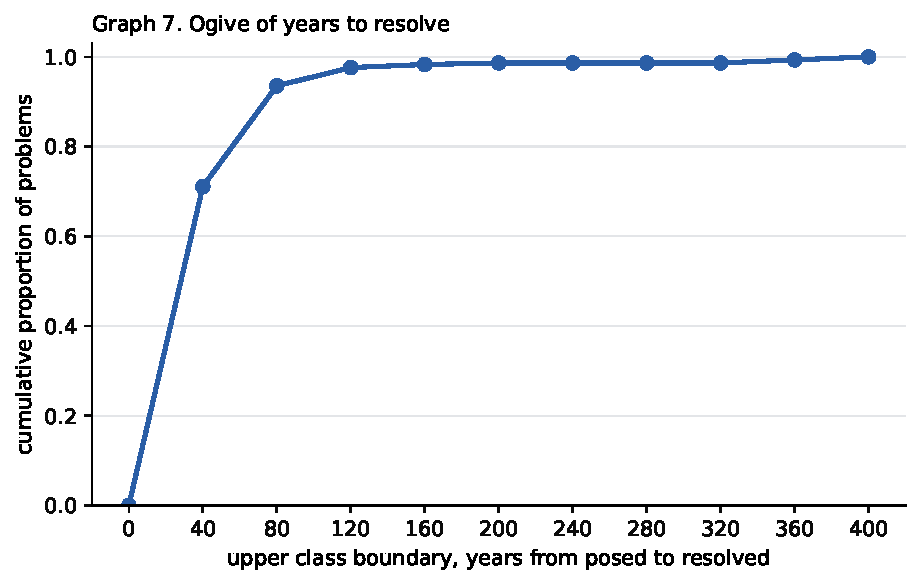
\includegraphics[width=0.82\linewidth]{figures/07-ogive.pdf}\end{center}
\noindent Graph 7: a proportion of 0.7109 of problems resolved in under 40 years and 0.9354 in under 80.


\begin{center}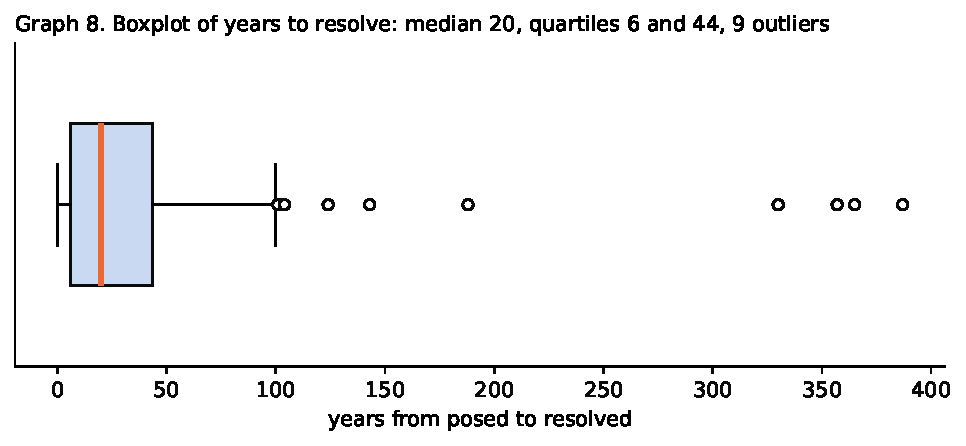
\includegraphics[width=0.82\linewidth]{figures/08-boxplot.pdf}\end{center}
\noindent Graph 8: the box runs from 6 to 44 years with the median at 20, and 9 points sit beyond the upper fence of 100.38.


\begin{center}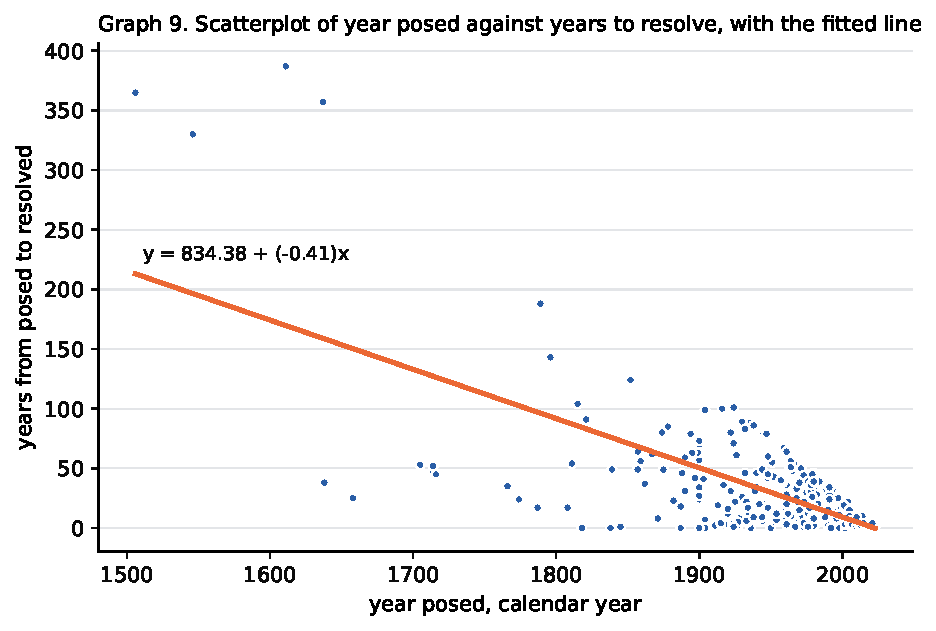
\includegraphics[width=0.82\linewidth]{figures/09-scatter.pdf}\end{center}
\noindent Graph 9: years to resolve fall as the posed year rises, $r = -0.67$.


\begin{center}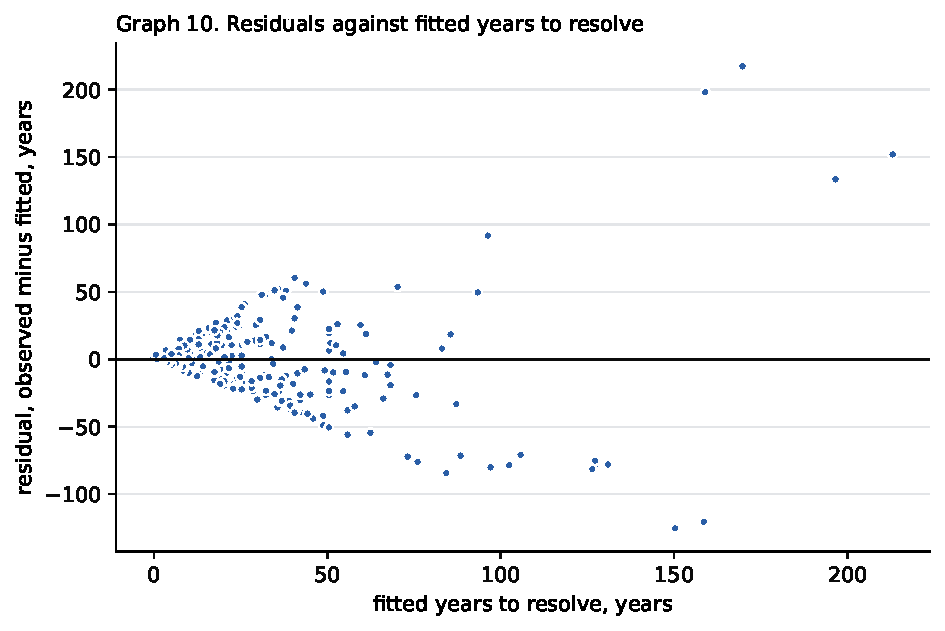
\includegraphics[width=0.82\linewidth]{figures/10-residuals.pdf}\end{center}
\noindent Graph 10: the residuals spread wider at large fitted values and have a hard lower edge, so the linear model's equal-spread assumption fails.


\begin{center}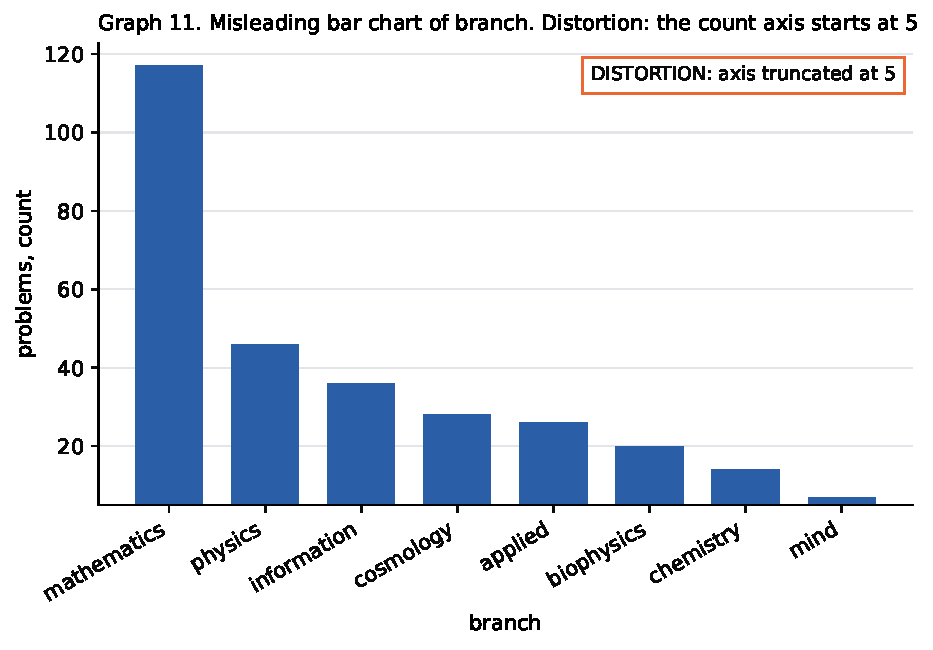
\includegraphics[width=0.82\linewidth]{figures/11-misleading.pdf}\end{center}
\noindent Graph 11: with the axis cut, the smallest branch looks close to empty and differences between branches look larger than they are.


\begin{center}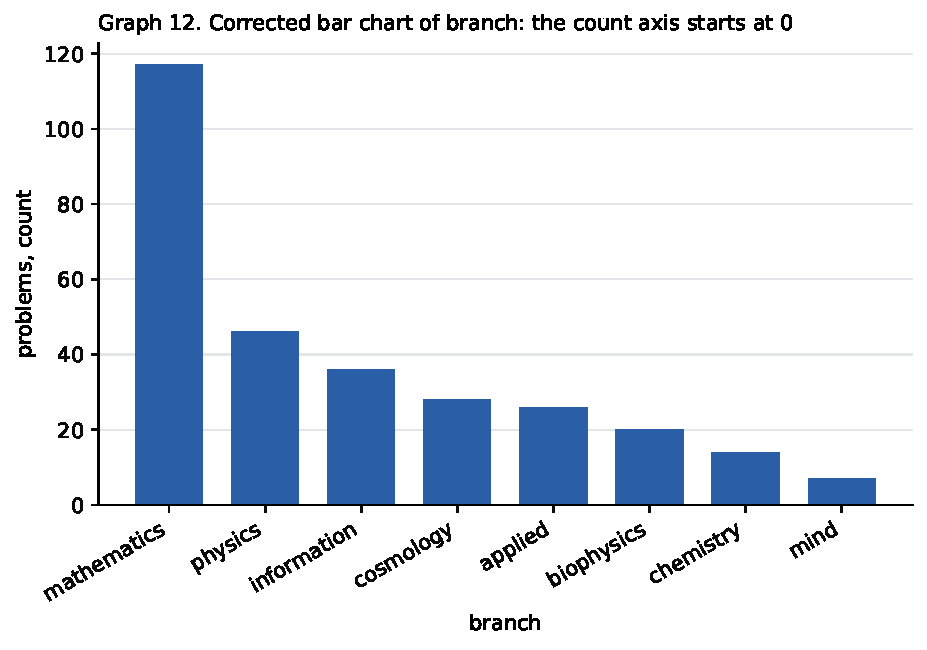
\includegraphics[width=0.82\linewidth]{figures/12-corrected.pdf}\end{center}
\noindent Graph 12: from a zero baseline the bar heights are proportional to the counts.


Shape: one cluster near zero, strong right skew, gaps above 200 years and 9 flagged values. The median, 20.00 years, is the main measure of centre, because the long right tail pulls the mean up to 31.71.

\section{Inferential Statistics}

\subsection{Probability}

Cutoff c = 50 years. A: a problem took at least 50 years. B: the problem is in physics.

\begin{center}\begin{tabular}{lrrr}
\toprule
 & A & not A & Total \\
\midrule
B & 7 & 39 & 46 \\
not B & 43 & 205 & 248 \\
Total & 50 & 244 & 294 \\
\bottomrule
\end{tabular}\end{center}

$P(A) = 50/294 = 0.1701$. $P(B) = 46/294 = 0.1565$. $P(A \text{ and } B) = 7/294 = 0.0238$. $P(A \text{ or } B) = 89/294 = 0.3027$. $P(A \mid B) = 7/46 = 0.1522$. $P(A)P(B) = 0.0266$, against $P(A \text{ and } B) = 0.0238$: the two differ by 0.0028, so A and B are close to independent in these data. $C(10,3) = 120$ counts the ways to choose which 3 of 10 draws are the successes.

\subsection{Models}

Binomial. K counts A-successes in 10 uniform draws with replacement, p = 0.1701. Conditions: a fixed number of 10 trials; two outcomes, A or not A; a constant p because draws are with replacement; independent draws. $P(K = 3) = C(10,3)\,p^3(1-p)^7 = 0.1601$. $P(K \ge 1) = 1 - (1-p)^{10} = 0.8450$. Mean $= 10p = 1.70$. SD $= \sqrt{10p(1-p)} = 1.19$.

Normal. Full-data mean $\mu = 31.71$ and population SD $\sigma = 47.07$ years. $P(Y \ge 50) = 0.3488$ under the model, against the observed proportion 0.1701. Modelled 90th percentile: 92.04 years, against 63.00 observed. The histogram is right-skewed and the model puts probability 0.2503 below zero years, so the fit is weak and these two results are model exercises.

\subsection{Sampling}

Reference population: all N = 294 cleaned rows, $\mu = 31.71$ and $\sigma = 47.07$ years. Method: \texttt{numpy.random.default\_rng(124).integers(1, N + 1, 50)} draws 50 independent uniform positions with replacement. Draws that repeat an earlier row: 0. Positions, row IDs and values are saved in \texttt{sample\_50.csv}.

Simulation: 500 samples of size 5 under seed 125 and 500 of size 50 under seed 126, separate from the saved sample. Every draw ID is in \texttt{simulation\_draws.csv} and all 1,000 means are in \texttt{simulation\_means.csv}.

\begin{center}\begin{tabular}{lrrrr}
\toprule
Sample size & Mean of means & SD of means & $\mu$ & $\sigma/\sqrt{n}$ \\
\midrule
n = 5 & 32.66 & 21.71 & 31.71 & 21.05 \\
n = 50 & 32.11 & 6.56 & 31.71 & 6.66 \\
\bottomrule
\end{tabular}\end{center}

\begin{center}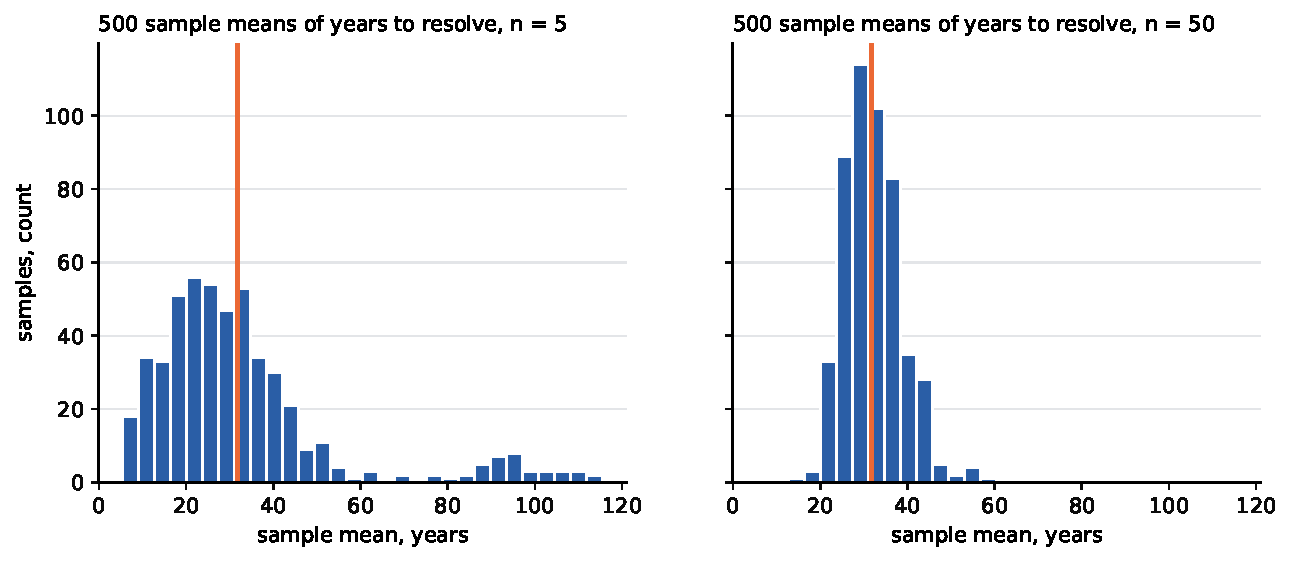
\includegraphics[width=0.82\linewidth]{figures/13-sampling.pdf}\end{center}
\noindent Both histograms centre near $\mu$, marked by the line. The spread shrinks from 21.71 at n = 5 to 6.56 at n = 50, close to $\sigma/\sqrt{n}$. At n = 5 the means keep the right skew of Y; at n = 50 the shape is closer to symmetric, as the central limit theorem predicts.


\subsection{Confidence Interval}

From the saved sample: n = 50, $\bar x = 22.32$, s = 23.22, SE $= 23.22/\sqrt{50} = 3.28$, df = 49, $t^* = 2.01$, margin $= 2.01 \times 3.28 = 6.60$. Interval: $22.32 \pm 6.60$, from 15.72 to 28.92 years.

Checks: the draws are independent by design. The sample is right-skewed, with median 17.00 and maximum 104 years, and n = 50 is large enough for the t procedure to be approximate; outliers widen the interval. Interpretation: we are 95\% confident that the mean time from posed to resolved for the 294 cleaned atlas problems is between 15.72 and 28.92 years. Across repeated samples of 50 drawn this way, about 95\% of the intervals built by this method would contain the reference mean. This interval misses the full-data mean of 31.71 years. The sample is kept as drawn.

\subsection{Hypothesis Test}

$H_0: \mu = 50$, $H_1: \mu \ne 50$, $\alpha = 0.05$. The benchmark of 50 years is hypothetical. $t = (22.32 - 50)/3.28 = -8.43$, df = 49, p-value $< 0.0001$. Decision: reject $H_0$. Conclusion: the sample provides evidence that the mean time to resolve differs from 50 years.

The decision agrees with the interval: 50 is outside 15.72 to 28.92. The p-value is the probability, when the mean is 50 years, of a sample mean at least this far from 50 in either direction. A Type I error would be concluding the mean differs from 50 years when it equals 50. A Type II error would be keeping 50 years when the mean differs. The sample mean minus the benchmark is $-27.68$ years, 55.36\% of the benchmark.

\section*{Analysis}
\noindent\fbox{\parbox{0.97\linewidth}{\textbf{DRAFT for Gianangelo to rewrite in his own words. Target 150 to 200 words.}}}

\medskip
Years from posed to resolved are right-skewed. Most solved problems in the atlas closed within a few decades: the median is 20.00 years and the third quartile is 43.75, while the mean is 31.71 because 9 problems sit beyond the upper fence of 100.38 years. The median is the better centre. Year posed and years to resolve move in opposite directions, with $r = -0.67$ and $R^2 = 0.45$; part of that slope comes from the table holding solved problems only, since a recent problem that is already solved has a short time by construction. The saved sample of 50 rows has mean 22.32 years, and its 95\% interval, 15.72 to 28.92, misses the full-data mean of 31.71. The test of the 50-year benchmark gives $p < 0.0001$, so the sample leads us to reject $H_0$. The sample mean differs from the full-data mean by $-9.39$ years, or 2.86 standard errors of 3.28.


\section*{Conclusion}
\noindent\fbox{\parbox{0.97\linewidth}{\textbf{DRAFT for Gianangelo to rewrite in his own words. Target 100 to 150 words.}}}

\medskip
The research question asks whether solved atlas problems took 50 years on average. The sample provides evidence against $H_0$: $t = -8.43$, $p < 0.0001$, and the interval runs from 15.72 to 28.92 years. Two limits apply. The table holds solved problems with both years recorded, so long-open problems that are still unsolved are missing and the mean understates how long problems stay open. The rows come from public lists that favour famous problems. One improvement: record a posed year for every row in the atlas, open or solved, so that open problems can enter as still running. The claim covers the 294 cleaned rows and no wider population of research problems.


\section*{References}

Bucket Foundation, Dichio, G. (2026). \emph{Solvability Atlas problem table}, version of 2026-10-13. \url{https://github.com/bucket-foundation/bucket-foundation/blob/dev/tools/solvability-atlas/surface/table.csv}. Accessed 2026-10-13.

Wikipedia contributors. Problem lists, science timelines and prize competition pages. CC BY-SA 4.0. The URL for each row is in \texttt{problems-sourced.tsv} in the atlas folder.

Google DeepMind. \emph{formal-conjectures}. Apache-2.0. \url{https://github.com/google-deepmind/formal-conjectures}.

Benchmark: $\mu_0 = 50$ years is hypothetical and has no outside source.

Software: Python with numpy, pandas, scipy and matplotlib; \texttt{stats\_project.py} reproduces every number under seed 124.

\end{document}